\documentclass[a4,11pt]{article}
\usepackage{tikz} %to draw models
\usetikzlibrary{tikzmark}
\usepackage{multicol} %for multi columns
\usepackage{xcolor} %for color
\usepackage[utf8]{inputenc}
\usepackage{gb4e}
\usepackage{enumitem}
\usepackage{amsmath} %for fractions
\usepackage{fullpage}
\usepackage{graphicx}
\graphicspath{ { } }


\setlength{\parindent}{0in}

\definecolor{Pink}{RGB}{240,0,120}
\newcommand{\jt}[1]{\textbf{\textcolor{Pink}{#1}}}


\title{Week 5: Quiz questions and model answers}
\author{Judith Tonhauser and Elena Vaik\v snorait\.{e} }
\date{\today}

\begin{document}

\maketitle

{\bf Introductory message:} This quiz covers the material in CC section 2.4. This section discusses licensing environments for negative polarity items (NPIs). This quiz test your knowledge of set theory (based on the previous chapter) and identifying whether an expression is downward entailing.

% An expression licenses NPIs wherever it licenses downward entailments (p.62)

% negative polarity items: defined as a word that is acceptable in a sentence with sentential negation but unacceptable in the positive variant
% distribution of NPIs: need to be able to talk about environments where NPIs are acceptable, e.g.,:
%	- argument of preposition
%	- clause-mate to adverb, 
%	- complement clause, 
%	- restriction of quantifier, scope of quantifier

% upward entailment, downward entailment
% semantic value of the NP musician is the set of musicians
% semantic value of the NP cellist ist the set of cellists
% subset relation, downward entailment

\begin{enumerate}[leftmargin = 12pt]

\item {\bf Euler diagram 1} A  the non-empty set of dogs. B is the non-empty set of all entities that like Whiskas. The meaning of which English sentence does the Euler diagram capture?


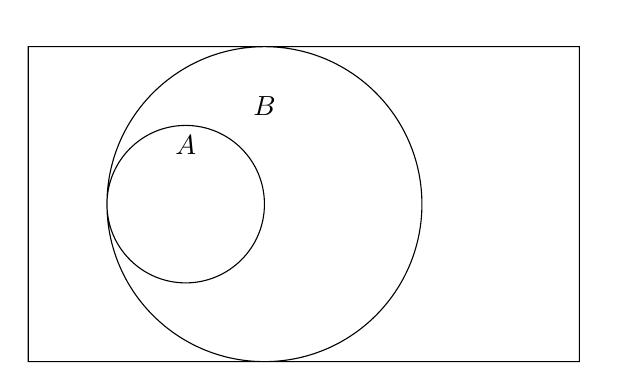
\begin{tikzpicture}
% outline, double numbers in parentheses are coordinates, single number is the size of the circle.
\draw (0,0) circle (1) (0,1)  node [text=black,below] {$A$}
         (1,0) circle (2) (1,1)  node [text=black,above] {$B$}
     (-2,-2) rectangle (5,2) node [text=black,above] {};
\end{tikzpicture}

      \begin{enumerate}[noitemsep]
        \item \textit{Some dogs like Whiskas.} (-1pt checked / 1pt unchecked)
	\item \textit{No dog likes Whiskas.} (-1pt checked / 1pt unchecked)
        \item \textit{Every dog likes Whiskas.} (1pt checked / -1pt unchecked)
	\end{enumerate}	


{\bf Model answer:}  The correct answer is \textit{Every dog likes Whiskas}, since every member of the set dog is also member of the set of entities that like Whiskas.

\item {\bf Euler diagram 2} A  the non-empty set of dogs. B is the non-empty set of all entities that like Whiskas. The meaning of which English sentence does the Euler diagram capture?

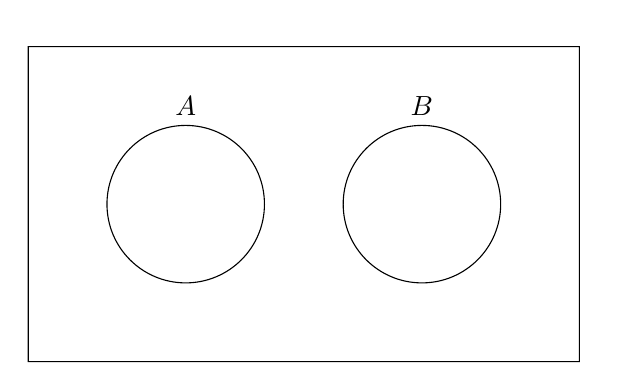
\begin{tikzpicture}
% outline
\draw (0,0) circle (1) (0,1)  node [text=black,above] {$A$}
         (3,0) circle (1) (3,1)  node [text=black,above] {$B$}
     (-2,-2) rectangle (5,2) node [text=black,above] {};
\end{tikzpicture}

      \begin{enumerate}[noitemsep]
        \item \textit{Some dogs like Whiskas.} (-1pt checked / 1pt unchecked)
	\item \textit{No dog likes Whiskas.} (-1pt checked / 1pt unchecked)
        \item \textit{Every dog likes Whiskas.} (1pt checked / -1pt unchecked)
	\end{enumerate}	


{\bf Model answer:}  The correct answer is \textit{No dog likes Whiskas}, since the intersection between the set of dogs and the set of entities that like Whiskas is empty.

\item {\bf Euler diagram 3} A  the non-empty set of dogs. B is the non-empty set of all entities that like Whiskas. The meaning of which English sentence does the Euler diagram capture?

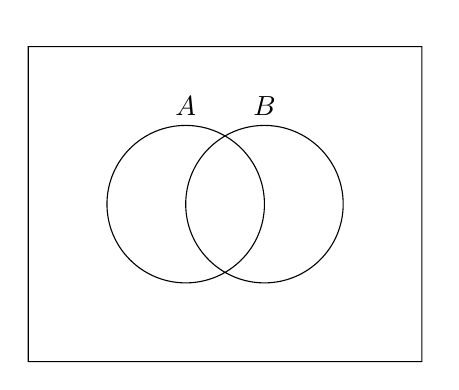
\begin{tikzpicture}
% outline
\draw (0,0) circle (1) (0,1)  node [text=black,above] {$A$}
      (1,0) circle (1) (1,1)  node [text=black,above] {$B$}
     (-2,-2) rectangle (3,2) node [text=black,above] {};
\end{tikzpicture}

      \begin{enumerate}[noitemsep]
        \item \textit{Some dogs like Whiskas.} (1pt checked / -1pt unchecked)
	\item \textit{No dog likes Whiskas.} (-1pt checked / 1pt unchecked)
        \item \textit{Every dog likes Whiskas.} (-1pt checked / 1pt unchecked)
	\end{enumerate}	

{\bf Model answer:}  The correct answer is \textit{Some dogs like Whiskas}, since the intersection between the set of dogs and the set of entities that like Whiskas is not empty.


\item {\bf Sets 1} A  the set of dogs. B is the set of all entities that like Whiskas. Which set theoretic formula captures the meaning of the sentence \textit{No dog likes Whiskas.}

      \begin{enumerate}[noitemsep]
        \item A $\cap$ B = $\emptyset$ (1pt checked / -1pt unchecked)
	\item A $\cup$ B = $\emptyset$  (-1pt checked / 1pt unchecked)
        \item A $\subset$ B (-1pt checked / 1pt unchecked)
	\end{enumerate}	
	
{\bf Model answer:}  The correct answer is  A $\cap$ B = $\emptyset$, since the intersection of dogs and likers of Whiskas is empty. 


\item {\bf Sets 2} A  the set of parrots. B is the set of all entities that like to sing. Which formula captures the meaning of the sentence \textit{Every parrot likes to sing.}

        \begin{enumerate}[noitemsep]
        \item A $\cap$ B = $\emptyset$ (1pt checked / -1pt unchecked)
	\item A $\cup$ B = $\emptyset$  (-1pt checked / 1pt unchecked)
        \item A $\subset$ B (-1pt checked / 1pt unchecked)
	\end{enumerate}	

{\bf Model answer:}  The correct answer is  A $\subset$ B because every member of the set of parrots is a member of the set of entities who like to sing.

\item {\bf Sets 3}  A is a set of dogs. B is a set of all entities that like Whiskas. C is a set of snorers. The following sentences are true. 

\begin{itemize}[noitemsep]
\item No dog likes Whiskas.
\item Some dogs are snorers.
\item Everyone who likes Whiskas is a snorer.
\end{itemize}

Select all true statements in set-theoretic notation. (Grading: multiple choice; 1pt if correct, -1pt if incorrect)

\begin{enumerate}
\item A $\cap$ B $\neq$ $\emptyset$
\item A $\cap$ B = $\emptyset$
\item A $\cap$ C $\neq$ $\emptyset$
\item A $\cap$ C = $\emptyset$
\item A $\subseteq$ C 
\item B $\subseteq$ C 
\item C $\subseteq$ B
\end{enumerate}

{\bf Model answer:} The correct answers are (b), (c), (f). (b) captures the sentence \textit{no dog likes Whiskas}, i.e. the intersection of dogs and entities that like Whiskas is empty. (c) captures the sentence \textit{some dogs are snorers}, i.e. the intersection of dogs and is not empty. (f) captures the sentence \textit{everyone who likes Whiskas is a snorer}.

(a) is false, it would be true if some dogs liked Whiskas. 
(d) is false, it would be true if no dog snored. 
(e) is false, it would be true if every dogs were a snorer. 
(g) is false, it would be true, if every snorer would like Whiskas.


\item {\bf Sets 4}  A is a set of humans. B is a set of all entities that like pizza. C is a set of all entities that like breadsticks.  The following sentences are true. 

\begin{itemize}[noitemsep]
\item Every person likes pizza.
\item Everyone who likes pizza likes breadsticks.
\end{itemize}

Select all true statements in set-theoretic notation. (Grading: multiple choice; 1pt if correct, -1pt if incorrect)

\begin{enumerate}
\item A $\subseteq$ B
\item A $\subseteq$ C
\item B $\subseteq$ C
\item B $\subseteq$ A
\item C $\subseteq$ A
\item C $\subseteq$ B
\end{enumerate}

{\bf Model answer:} The correct answers are (a), (b), (c). (a) and (c) correspond to the above given sentences. (b) is true because A is a subset of B and B is a subset of C, therefore A is a subset of C.

\item {\bf Monotonicity: Every} The quantifier \textit{every} is left downward monotone. Given the sentence \textit{Every human uses Twitter}, write an argument that \textit{every} is left downward monotone. Make sure that your argument includes a relevant version of the sentence and explicit states how the two sentences show that \textit{every} is left downward monotone. (23points, max 250 characters)
	
{\bf Model answer:} Consider the sentence \textit{Every woman uses Twitter}, where \textit{human} has been replaced by an expression that denotes a subset of humans, namely \textit{woman}. Because \textit{Every human uses Twitter} entails \textit{Every woman uses Twitter}, \textit{every} is left downward monotone. (1 point for a correct version of the sentence, 1 point for statement about the entailment relationship, 1 point for the  )

\item {\bf Monotonicity: No/Few/All} 

\begin{enumerate}
\item The quantifier \textit{no} is right downward monotone because the sentence \textit{No dog likes to sleep} entails:

      \begin{enumerate}[noitemsep]
        \item \textit{No dog likes to sleep on the ground} (1pt checked / -1pt unchecked)
	\item \textit{No poodle likes to sleep} (-1pt checked / 1pt unchecked)
        \item \textit{Noone likes to sleep} (-1pt checked / 1pt unchecked)
	\end{enumerate}	

\item  Based on the sentences below, determine whether \textit{few} is downward monotone. Select all that apply. 

\begin{itemize}[noitemsep]
\item Few athletes play piano.
\item Few footballers play piano.
\item Few athletes play piano well.
\end{itemize}

      \begin{enumerate}[noitemsep]
        \item Left downward monotone (1pt checked / -1pt unchecked)
        \item Right downward monotone (1pt checked / -1pt unchecked)
        \item Not downward monotone (-1pt checked / 1pt unchecked)
	\end{enumerate}	

\item Based on the sentences below, determine whether \textit{all} is downward monotone. Select all that apply. 
\begin{itemize}[noitemsep]
\item All dogs love walks.
\item All chihuahuas love walks.
\item All dogs love walks in a park.
\end{itemize}


      \begin{enumerate}[noitemsep]
        \item Left downward monotone (1pt checked / -1pt unchecked)
        \item Right downward monotone (-1pt checked / 1pt unchecked)
        \item Not downward monotone (-1pt checked / 1pt unchecked)
	\end{enumerate}	

\end{enumerate}



{\bf Model answers:}
\begin{enumerate}
 \item The correct answer is \textit{No dog likes to sleep on the ground}. A right downward monotone determiner is a determiner such that in a sentence of the form D X Y it entails D X Y', where Y' is a subset of Y. \textit{Sleep on the ground} is a subset of \textit{sleep}. The sentence \textit{No poodle likes to sleep} shows that \textit{no} is also left downward monotone, because a poodle is a subset of dogs.

\item The correct answers are left and right downward monotone. If \textit{Few athletes play piano} is true, then it means that \textit{few footballers play piano.} is also true. Since footballers is a subset of athletes, few is left downward monotone. If \textit{Few athletes play piano} is true, then it is also true that \textit{few athletes play piano well}, since the set containing all entities that play piano well is a subset of  the set that contains all entities that play piano.

\item The correct answer is left downward monotone. If \textit{All dogs love walks} is true, then it means that \textit{all chihuahuas love walks} is also true. Since chihuahuas is a subset of dogs, \textit{all} is left downward monotone. If \textit{All dogs love walks} is true, it does not entail that \textit{all dogs love walks in a park} is true. Some dogs might prefer walks in a city center. Therefore, \textit{all} is not right downward monotone.
\end{enumerate}


\item {\bf Licensing of negative polarity items} According to Ladusaw 1980, in which linguistic environments are negative polarity items licensed, i.e., in which linguistic environments are they acceptable?  

  \begin{enumerate}[noitemsep]
        \item NPIs are acceptable in downward monotone environments. (1pt)
        \item NPIs are acceptable in upward monotone environments. (0pts)
	\end{enumerate}

{\bf Model answer:} As discussed on p.62, answer (a) is correct. The Fauconnier-Ladusaw generalization is that ``an expression licenses negative polarity items wherever it licenses downward entailments''.

\item {\bf Downward monotonicity} (question pool)

\begin{enumerate}[noitemsep]

\item Show that the argument of \textit{without} is a downward entailing environment. (The determiner phrase \textit{any help} is the argument of \textit{without}.) (4 points; max. 550 characters)

\item Show that the argument of \textit{hard} is a downward entailing environment. (In the sentence \textit{It is hard to buy a Mercedes}, the \textit{to}-infinitive \textit{to buy a Mercedes} is the argument of \textit{hard}.) (4 points; max. 550 characters)

\end{enumerate}

{\bf Model answers:} 

\begin{enumerate}[noitemsep]

\item To show that the argument of \textit{without} is a downward entailing environment, consider the two sentences \textit{Kim runs without wolves} and \textit{Kim runs without animals}. These two sentences differ only on the argument of {\em without}: {\em animals} denotes a superset of {\em wolves}. Because \textit{Kim runs without animals} entails \textit{Kim runs without wolves}, the argument of \textit{without} is a downward entailing environment, i.e., the argument licenses entailments from supersets to subsets.  (1 point each for the two sentences, 1 point for statement about entailment relationship, 1 point for concluding statement)

\item To show that the argument of \textit{hard} is a downward entailing environment, consider the two sentences {\em It is hard to run} and {\em It is hard to run fast}. These two sentences differ only on the argument of {\em hard}: the set denoted by {\em to run} is a superset of the set denoted by {\em to run fast}. Because {\em It is hard to run} entails {\em It is hard to run fast}, the argument of {\em hard} is a downward entailing environment, i.e., the argument licenses entailments from supersets to subsets. (1 point each for the two sentences, 1 point for statement about entailment relationship, 1 point for concluding statement)

\end{enumerate}

\item {\bf Upward monotonicity} (question pool)

\begin{enumerate}[noitemsep]

\item Show that the argument of \textit{with} is an upward entailing environment. (In (4a), the determiner phrase \textit{any help} is the argument of \textit{with}.) (4 points; max. 550 characters)

\item Show that the argument of \textit{easy} is an upward entailing environment. (In the sentence \textit{It is easy to buy a Mercedes}, the \textit{to}-infinitive \textit{to buy a Mercedes} is the argument of \textit{easy}.) (4 points; max. 550 characters)

\end{enumerate}

{\bf Model answers:} 

\begin{enumerate}[noitemsep]

\item To show that the argument of \textit{with} is an upward entailing environment, consider the two sentences \textit{Kim runs with wolves} and \textit{Kim runs with animals}. These two sentences differ only on the argument of {\em with}: {\em animals} denotes a superset of {\em wolves}. Because \textit{Kim runs with wolves} entails \textit{Kim runs with animals}, the argument of \textit{with} is an upward entailing environment, i.e., the argument licenses entailments from subsets to supersets. (1 point each for the two sentences, 1 point for statement about entailment relationship, 1 point for concluding statement)

\item To show that the argument of \textit{easy} is an upward entailing environment, consider the two sentences {\em It is easy to run fast} and {\em It is easy to run}. These two sentences differ only on the argument of {\em easy}: the set denoted by {\em to run} is a superset of the set denoted by {\em to run fast}. Because {\em It is easy to run fast} entails {\em It is hard to run}, the argument of {\em easy} is an upward entailing environment, i.e., the argument licenses entailments from subsets to supersets. (1 point each for the two sentences, 1 point for statement about entailment relationship, 1 point for concluding statement)

\end{enumerate}


\end{enumerate}
\end{document}
